\chapter{Animations}
De class \eeClass{Game.Chr} voorziet een aantal standaard animaties. Die zijn echter zelden genoeg. In dit hoofdstuk zie je hoe je deze animaties aanpast, en hoe je nieuwe animaties toevoegt.

Esenthel maakt een onderscheid tussen standaard animaties and custom animaties. De standaard animaties worden automatisch toegepast aan de hand van enkele variabelen in \eeClass{Game.Chr}. Als je de header file van deze class opent, dan zie je binnen de class een struct \eeClass{Input}. Deze class regelt hoe je avatar over het scherm beweegt. Je ziet properties zoals crouch, walk, jump en dodge.

Het is eenvoudig om deze waarden aan te passen. Je hebt dat trouwens al gedaan in een van de vorige hoofdstukken. Denk aan code zoals:

\begin{code}
input.turn.x = Kb.b(KB_Q) - Kb.b(KB_E);
input.turn.y = Kb.b(KB_T) - Kb.b(KB_G);
input.move.x = Kb.b(KB_D) - Kb.b(KB_A);
\end{code}

\section{Player Animations}

\begin{exercise}
De avatar heeft, naast een run animatie, ook een walk animatie. Die wordt op dit moment niet gebruikt. Pas de code in \eeFunc{player.update} aan zodat je avatar standaard wandelt, maar wel loopt wanneer de linker ctrl toets ingedrukt is. Zoek in de struct \eeClass{Input} op welke property je hier voor aanpast.
\end{exercise}

\section{Jump}
Vreemd genoeg bevat \eeClass{Input} wel een property jump die de avatar tijdelijk omhoog beweegt, maar bestaat er geen standaard animatie voor jump. Dat wil zeggen dat je een custom animatie moet gebruiken. Om dit te doen heb je een \eeClass{Motion} object nodig. Voeg alvast dit object toe aan de class \eeClass{Player}.

\begin{code}
Motion jumpMotion;
\end{code}

In de functie \eeFunc{update} kan je de huidige `jump' code aanvullen:

\begin{code}
// jumping
input.jump = Kb.bp(KB_SPACE) ?  3.5 :  0;
if(Kb.bp(KB_SPACE))
{
  jumpMotion.set(skel, === drop jump animation ===);
}
jumpMotion.updateAuto(5, 5, 1);
\end{code}

Het eerste statement stond al in je code. Dat bepaalt of je avatar al dan niet even omhoog gaat. Daarna stel je de animatie in wanneer de speler op de spatiebalk drukt. Het eerste argument is het skeleton waarop de animatie van toepassing is. De waarde `skel' is skeleton dat al aanwezig is in \eeClass{Game.Chr}. Het tweede argument is de verwijzing naar de animatie. Drop daar de jump animatie die je vindt in Assets $\Rightarrow$ characters $\Rightarrow$ samurai.

Tijdens elke update moeten ook alle \eeClass{Motion} object geupdated worden. In dit geval is dat jumpMotion. Je kan de \eeFunc{updateAuto} functie gebruiken om het eenvoudig te houden. De eerste twee argumenten bepalen hoe snel je overschakelt van de standaard animatie naar de jump animatie en omgekeerd. Het derde argument is de algemene snelheid waarmee de animatie getoond wordt.

Wanneer je nu de game uitvoert, zal je zien dat de jump animatie niet gebruikt wordt. We moeten eerst de aanwezige functie \eeFunc{animate} van \eeClass{Game.Chr} overschrijven. Die functie voert nu enkel de standaard animaties uit. Omdat dit een virtuele functie is (kijk in de header file!) moet je daarin ook de oorspronkelijke functie uitvoeren. \textit{(Tenzij je echt niet wil dat de standaard animaties gebruikt worden.)} Voeg daarom de volgende functie toe aan je player class:

\begin{code}
virtual void animate()
{
  super.animate();
  skel.animate(jumpMotion, true);
}
\end{code}

Deze functie voert eerst de standaard animaties uit. Daarna wordt de \eeClass{jumpMotion} toegevoegd. Het extra argument `replace' bepaalt dat de vorige animaties overschreven moeten worden. Wanneer je `false' gebruikt, zal de impact van de vorige animaties veel groter zijn.

\begin{exercise}
Pas de waarden in \eeFunc{updateAuto} aan een bekijk het resultaat. Bekijk ook hoe anders de animatie is wanneer je \eeFunc{skel.animate(jumpMotion, false)} gebruikt.

Voeg een extra \eeClass{Motion} `attackMotion' toe aan de \eeClass{player} class. In de asset list zie je drie attacks: `attack\_double', `attack1' en `attack2'. Zorg er voor dat `attack\_double' uitgevoerd wordt wanneer je de F toets indrukt. Wanneer je de R toets indrukt kiest je programma zelf tussen `attack1' en `attack2'.
\end{exercise}

\section{The Butterfly Effect}
Het demo project bevat ook een vlinder. Om niet voor elk dier een afzonderlijke game class te moeten maken, bevat het project een enum \eeClass{ANIMAL} en een object class \eeClass{OBJ\_ANIMAL}. De object class bevat een animatie en een enum type. Het Butterfly object heeft dan weer deze class als parameter, zodat je de default waarden kan aanpassen voor andere dieren.

Om de vlinders zichtbaar te maken in je game, maak je zoals altijd een class aan. We gaan er van uit dat alle dieren kunnen bewegen, dus wordt de class afgeleid van \eeClass{Game.Chr}. De basis voor de class ziet er zo uit:

\begin{code}
class animal : Game.Chr
{
	ANIMAL animalType;

	// for the butterfly
	Vec startPos;
	float timer = 0;

	virtual void create(Object & obj) {
		super.create(obj);
	}

	virtual bool update() {
		bool result = super.update();

		// add your own code

		return result;
	}
}
Game.ObjMap<animal> Animals;
\end{code}

Vergeet niet deze class aan je \eeClass{Game.World} toe te voegen bij het laden van de wereld. Daarna start je de game en zie je de vlinders in actie. Nu ja, veel actie is er niet. Ze blijven stil zitten. Tijd om daar wat aan te doen.

Ten eerste dien je het type van het dier uit de object parameters te halen, zodat je weet met wat je te maken hebt. (Momenteel zijn het allemaal vlinders, maar dat zal in een grotere game wel anders zijn.) Je zou ondertussen zelf moeten weten in welke lidfunctie van animal je de onderstaande code toevoegt:

\begin{code}
animalType = (ANIMAL)obj.getParam("type").asEnum();
\end{code}

Eenmaal je het \eeClass{animalType} hebt, kan je enkele instellingen voor de vlinder klaarzetten:

\begin{code}
if(animalType == A_BUTTERFLY)
{
 	startPos = pos();
 	ctrl.flying(true);
}
\end{code}

De redenen voor deze regels zijn de volgende:
\begin{itemize}
	\item We willen de huidige positie onthouden als de startPositie. Als we later de vlinder telkens een nieuwe positie geven, en we weten niet waar hij oorspronkelijk was, dan kan de vlinder uiteindelijk eender waar terecht komen. Met een start positie kunnen we steeds in de buurt van de oorspronkelijke plaats blijven.
	\item De meeste dieren (en mensen) vliegen niet. Dat betekent dat ze nooit de weg zullen vinden naar een positie in de lucht. Een vlinder willen we toch vooral in de lucht zien, dus we stellen dat in via de skeleton controller.
\end{itemize}

In de update functie gaan we nu met hulp van een timer regelmatig een nieuwe doelpositie aan de vlinder toewijzen. Zo lijkt het alsof het beest doelloos rondvliegt, net zoals je van een vlinder verwacht.

\begin{code}
if(animalType == A_BUTTERFLY)
{
 	timer -= Time.d();
 	// move around a bit
 	if(timer < 0)
 	{
    	Vec targetPos = startPos;
	    targetPos.x += RandomF(-2, 2);
	    targetPos.y += RandomF(.1, 1);
	    targetPos.z += RandomF(-2, 2);
	    actionMoveTo(targetPos);
	    
	    flying_speed = 1;
	    anim.speed = 1;
	    timer = 1;
 	}
}
\end{code}

\begin{exercise}
Pas de waarden van \eeClass{flying\_speed}, \eeClass{anim.speed} en \eeClass{timer} aan met een random functie om de beweging nog echter te maken.

Het demo project bevat ook sardines. Schrijf zelf de code om die te laten bewegen. Een vis beweegt meestal wel door het water, dus de y positie kan je als volgt bepalen:

\begin{code}
targetPos.y = RandomF(Game.World.hmHeight(targetPos.xz()), -1);
\end{code}

\end{exercise}

\section{Walking with Dinosaurs}
In dit onderdeel voeg je een tweede dier toe: een dinosaurus. Maar voor we met de code beginnen zijn er enkele zaken in de editor die de moeite zijn om eens te bekijken.

\subsection{Material Variations}

Wanneer je de Dinosaur in de navigator uitklapt, dan zie je dat die drie verschillende materialen voorziet. Open het object in de object editor en kies het tabblad `Variations'. Daar zie je dat er drie variaties bestaan: Default, red en blue. Het gebeurt vaak in een game dat er meerdere versies van een object bestaan. Zo kan je een model herbruiken en via de materialen toch variaties aanbrengen. 

Open daarna de world editor en ga op zoek naar de dinosaurus. Wanneer je die selecteert (met het tabblad Object geopend) dan zie je ook daar de keuze `Variation'. Via deze droplist kan je op een eenvoudige manier de gewenste variatie kiezen.

\begin{figure}[h]
\centering
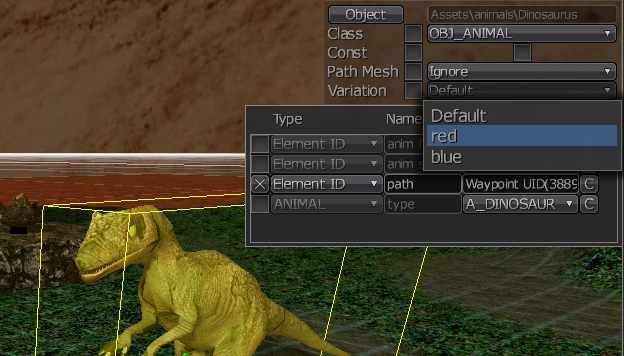
\includegraphics[width=0.8\linewidth]{../images/meshVariations.png}
\caption[]{Object Variations}
\label{fig:objectVariations}
\end{figure}

\subsection{Waypoints}

Een ander nieuw element zie je via de tab `Waypoint'. Waypoints bestaan uit \'e\'en of meerdere co\"ordinaten die je kan oproepen via code. In dit geval willen we de dinosaurus laten lopen volgens een vaste route. We voegen daarom 5 co\"ordinaten toe aan de wereld. De naam is vooral handig om Waypoints in de editor te herkennen. Omdat de dinosaurus dient rond te lopen, kiezen we als loop mode `Loop'. Daarna kan je de ID copi\"eren. 

Tot slot kan je terug naar de tab `Object' waar je de dinosaurus selecteert. Om je waypoint aan een object te linken, kan je een nieuwe parameter toevoegen. (Dat is voor deze dinosaurus al in orde.) Deze parameter wordt een Element ID, waarna je de ID kan plakken als waarde.

\begin{figure}[h]
\centering
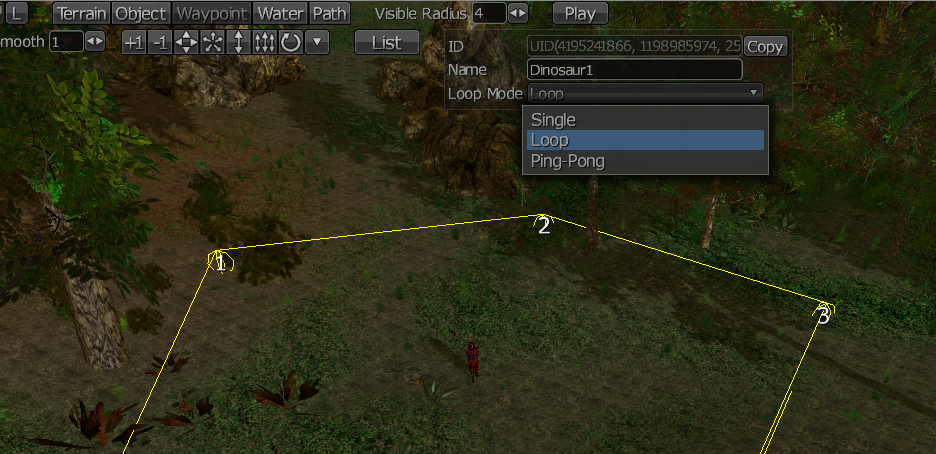
\includegraphics[width=0.8\linewidth]{../images/waypoints.png}
\caption[]{Waypoints}
\label{fig:waypoints}
\end{figure}

\subsection{Steps}
Open de animatie Assets $\Rightarrow$ animals $\Rightarrow$ Dinosaur $\Rightarrow$ walk. Controleer eerst of de optie `Loop' aangevinkt staat. Wanneer dat niet het geval is, dan gebeurt de loop enkel in de editor, maar nooit in je game. Het lijkt dan alsof de animatie niet werkt, tenzij je recht naar het object kijkt wanneer de game start.

Animaties kunnen events bevatten. Die events worden in je game gebruikt om functies uit te voeren wanneer de animatie zich op dat punt bevindt. Om de naam van de aanwezige events te zien, druk je onderaan op de knop Rename. Je ziet dat de animatie twee events bevat met de naam step. Step events worden automatisch herkend in je game en voeren een virtuele functie uit die je kan overschrijven (dadelijk meer daarover). Je kan aan elke animatie step events toevoegen, meestal om het geluid van een voetstap af te spelen.

\subsection{Code}

Een dinosaurus heeft, net zoals een vlinder, de object class \eeClass{OBJ\_ANIMAL}. Dat betekent dat je er geen nieuwe class voor moet maken. We gebruiken de class \eeClass{animal}. Die class moet dan wel aangepast worden, zodat zowel vlinders als dino's op een logische manier kunnen bewegen. Daarom voegen we eerst enkele variabelen toe aan de class:

\begin{code}
// for the dinosaur
Game.Waypoint * path = null;
int currentPointInPath = 0;
\end{code}

De eerste waarde is een pointer naar een waypoint. We stellen de pointer gelijk aan null, dus by default heeft een dier geen path. Om een dier met een path rond te laten lopen, moeten we onthouden wat het huidige doel is. Dat gebeurt via \eeClass{currentPointInPath}.

Vervolgens breid je de \eeFunc{create} functie uit:

\begin{code}
if(obj.findParam("path") != null)
{
 	path = Game.World.findWaypoint(obj.getParam("path").asID());        
}

if(animalType == A_DINOSAUR)
{
 	sac.stand = skel.getSkelAnim(== drop Assets/animals/Dinosaur/idle ==));
 	sac.walk = skel.getSkelAnim(== drop Assets/animals/Dinosaur/idle ==));
 	move_walking = true;
}
\end{code}

In het eerste deel gaan we op zoek naar een parameter `path'. De functie \eeFunc{findParam} heeft als resultaat null wanneer die parameter niet aanwezig is. Wanneer het resultaat niet null is, kan je die als ID doorgeven aan \eeFunc{Game.World.findWaypoint}. Nu krijg je als resultaat een pointer naar het betreffende waypoint. Die gebruiken we later als path voor het object.

In het tweede deel van de code stellen we enkele animaties in wanneer \eeClass{animalType} gelijk is aan \eeClass{A\_DINOSAUR}. Deze animaties zullen automatisch gebruikt worden wanneer de dinosaurus door de wereld beweegt. Bovendien stellen we \eeClass{move\_walking} gelijk aan true. Wanneer je dat niet doet, zal er gezocht worden naar een `run' animatie, die hier niet bestaat.

Nu kan je het gedrag van de dinosaurus bepalen in de update functie. Om het eenvoudig te houden gebruiken we een timer. Elke twintig seconden laten we de dinosaurus naar een volgend punt in het path wandelen.

\begin{code}
if(animalType == A_DINOSAUR && path != null)
{
 	timer -= Time.d();
 	if(timer < 0)
 	{
    	currentPointInPath++;
    	if(currentPointInPath == path.points.elms())
    	{
       		currentPointInPath = 0;
    	}
    	actionMoveTo(path.points[currentPointInPath].pos);
    	timer = 20;
 	}         
}
\end{code}

De timer logica zou je ondertussen wel bekend moeten zijn, en ook de rotatie doorheen de beschikbare punten heb je al eerder gebruikt. Nieuw is de functie \eeFunc{actionMoveTo}, die we gebruiken om de positie van het huidige punt als doel in te stellen.

Tot slot nog \'e\'en extra functie: \eeFunc{animateStepOccured}. Dit is een virtuele functie die de engine uitvoert wanneer een een `stap' gezet wordt. Meestal gebruik je die om het geluid van een voetstap te spelen. In dit geval gebruik je een versie van \eeClass{SoundPlay} die een geluid op een 3D positie afspeelt. Deze versie heeft ook een `range' argument waarmee je bepaalt tot op welke afstand het geluid hoorbaar is (hier 50 meter).

\begin{code}
virtual void animateStepOccured()
{
  SoundPlay(=== drop Sound/dino_step ===, 	// sound
  			pos(), 							// position
  			50, 							// range
  			RandomF(0.5, 1.0), 				// volume
  			VOLUME_FX, 						// channel
  			RandomF(0.8, 1.2)				// speed
  );
}
\end{code}

\begin{note}
Meestal schrijf je een functie op een enkele regel, maar dat is niet verplicht. Wanneer functies veel argument of een complexe berekening bevatten, is het vaak overzichtelijker om elk argument op een afzonderlijke regel te plaatsen.
\end{note}

\begin{exercise}
Met de nieuwe informatie in dit hoofdstuk kan je heel wat beweging in je game voorzien. Neem je tijd extra animals (vlinders en dino's) aan je project toe toe voegen. Experimenteer ook met de update code om het gedrag van elk dier aan te passen. 

Schrijf tot slot ook code om de kitten (al aanwezig in het project) over zijn path te laten bewegen.
\end{exercise}